\problemname{Logic Puzzle}

While browsing a kiosk at a recent trip, you bought a magazine filled
with various kinds of logic puzzles.
After a while of solving, however, you start to get a bit bored of the
puzzles.
Still wanting to complete all the puzzles in the magazine, you start
wondering about ways to solve some of them algorithmically.

The puzzle you are currently trying to solve is called \emph{Mosaic}, and
it is quite similar to the classic \emph{Minesweeper} video game:

\begin{figure}[!h]
  \centering
  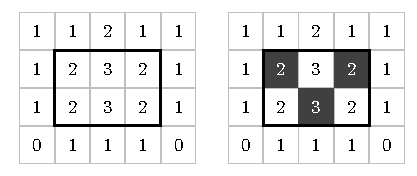
\includegraphics[width=.7\textwidth]{mosaic}
  \caption{Illustration of the first sample}
\end{figure}

You are given a two-dimensional grid of cells, initially all white,
and you have to color some of the cells in black.
You are also given a grid of clue numbers, which extends beyond the
borders of the puzzle grid by one cell in each direction.
The number in a cell indicates (exactly) how many cells in the
$3\times3$ block centered at this cell need to be colored in black.
You may not color any cells outside of the original grid.

\section*{Input}

The input consists of:
\begin{itemize}
  \item one line with two integers $h,w$ ($1 \le h,w \le 100$),
    the height and width of the puzzle;
  \item $h+2$ lines, each with $w+2$ integers $c_1,\dots,c_{w+2}$ ($0 \le c_i \le 9)$,
    the clue numbers.
\end{itemize}

\section*{Output}

If the given clue numbers are inconsistent, output \texttt{impossible}.
Otherwise, output $h$ lines with $w$ characters each, the solution to
the puzzle. Use \texttt{X} for black cells and \texttt{.} for white
cells.
If there are multiple solutions, any of them will be accepted.
